%% REPLACE SXXXXXX with your student number
\def\studentNumber{S2156578}


%% START of YOUR ANSWERS
%% Add answers to the questions below, by replacing the text inside the brackets {} for \youranswer{ "Text to be replaced with your answer." }. 
%
% Do not delete the commands for adding figures and tables. Instead fill in the missing values with your experiment results, and replace the images with your own respective figures.
%
% You can generally delete the placeholder text, such as for example the text "Question Figure 2 - Replace the images ..." 
%
% There are 18 TEXT QUESTIONS (a few of the short first ones have their answers added to both the Introduction and the Abstract). Replace the text inside the brackets of the command \youranswer with your answer to the question.
%
% There are also 3 "questions" to replace some placeholder FIGURES with your own, and 3 "questions" asking you to fill in the missing entries in the TABLES provided. 
%
% NOTE! that questions are ordered by the order of appearance of their answers in the text, and not by the order you should tackle them. Specifically, you cannot answer Questions 2, 3, and 4 before concluding all of the relevant experiments and analysis. Similarly, you should fill in the TABLES and FIGURES before discussing the results presented there. 
%
% NOTE! If for some reason you do not manage to produce results for some FIGURES and TABLES, then you can get partial marks by discussing your expectations of the results in the relevant TEXT QUESTIONS (for example Question 8 makes use of Table 1 and Figure 2).
%
% Please refer to the coursework specification for more details.


%% - - - - - - - - - - - - TEXT QUESTIONS - - - - - - - - - - - - 



%% Question 1:
\newcommand{\questionOne} {
\youranswer{
    % Question 1 - Explain what these figures contain and how the curves evolve, and spot where overfitting occurs. Reason based on the min/max points and velocities (direction and magnitude of change) of the accuracy and error curves
    the training data accuracy increases as the epoch number increases and for the validation data the accuracy stagnates at one point and slowly decreases as the epoch increases. In Figure 1b the training data error decreases as the epoch number increases and the validation data error decreases until about 12-14 epochs and start to increase rapidly as the epoch increases. The reason behind this is due to the overfitting of the training data as the model adapts too much of the training data. The point when overfitting occurs is about at the maximum accuracy by epoch and the minimum point of the error by epoch on the validation data, which is about between 12 to 14 epochs. 
    }
}

%% Question 2:
\newcommand{\questionTwo} {
\youranswer{
    % Question 2 - Present your network width experiment results by using the relevant figure and table
    with an increase in amount of hidden layers from 32 to 64 to 126 the training data accuracy increases and the training data error decreases no matter the number of epochs. In terms of the accuracy for the validation data, the maximum accuracy we can achieve increases with amount of hidden layers, but as overfit the training data (increasing the epoch), the accuracy declines at a faster rate as the number of hidden layers increases. For the error for validation data, again the minimum error we achieve decreases with the increase in hidden layers, but the rate of error increasing after the point where overfitting starts to occur, increases as the amount of hidden layers increase. And eventually the accuracy of validation data for 128 hidden layers would be below the accuracy of validation data for 32 hidden layers, and the error of validation data for 128 hidden layers would be higher the error of validation data for 32 hidden layers.
    }
}

%% Question 3:
\newcommand{\questionThree} {
\youranswer{
    % Question 3 - Discuss whether varying width affects the results in a consistent way, and whether the results are expected and match well with the prior knowledge (by which we mean your expectations as are formed from the relevant Theory and literature)
    Varying the network width affects results consistently, aligning with theoretical expectations. As hidden units increase, the model improves on training data but becomes more prone to overfitting. This leads to faster degradation in validation performance as the network size grows. While larger models initially improve validation accuracy, they decline more rapidly with longer training, which is expected due to the increased risk of overfitting in wider networks.
    }
}

%% Question 4:
\newcommand{\questionFour} {
\youranswer{
    % Question 4 - Present your network depth experiment results by using the relevant figure and table
    the difference between having one hidden layer and 2 hidden layers is pretty significant, we an constant higher training accuracy and constant lower training error, regardless of the number of epochs. In contrast, the training accuracy and error for models with two and three hidden layers are very similar, showing minimal differences. When looking at the validation data, the maximum validation accuracy for one hidden layer is noticeably lower than that of two hidden layers. However, the maximum validation accuracy for the model with three hidden layers is roughly the same as that of the two hidden layers one. The rate at which validation accuracy decreases is generally similar across the models, but the two hidden layers show a slightly faster decline. Regarding validation error, the model with one hidden layer has a higher minimum validation error, but it also shows a significantly lower rate of increase in validation error. Both the two and three hidden layer models have similar minimum validation errors, although the three hidden layer model has a slightly higher rate of increase in validation error over time.
    }   
}

%% Question 5:
\newcommand{\questionFive} {
\youranswer{
    % Question 5 - Discuss whether varying depth affects the results in a consistent way, and whether the results are expected and match well with the prior knowledge (by which we mean your expectations as are formed from the relevant Theory and literature)
    
Varying the depth of neural networks shows consistent and expected results in line with deep learning theories. The substantial increase in training accuracy and decrease in error when moving from one to two hidden layers reflects improved capacity for learning complex patterns. However, the minimal performance differences between two and three layers illustrate diminishing returns, indicating that additional depth offers limited benefits.
The notable rise in maximum validation accuracy from one to two layers contrasts with the similar performance of two and three layers, suggesting that extra depth may not significantly enhance generalization. The higher minimum validation error for the one-layer model indicates it struggles to capture data distributions effectively. Overall, while increasing depth can enhance performance, it may also risk overfitting, thereby constraining the advantages of added layers.
    }
}





%% Question 6:
\newcommand{\questionSix} {
\youranswer{Question 6 - Explain the experimental details (e.g. hyperparameters), discuss the results in terms of their generalisation performance and overfitting. Select and test the best performing model as part of this analysis.}
}

%% Question 7:
\newcommand{\questionSeven} {
\youranswer{Question 7 - Assume you were able to run 8 further training instances (8 specific hyperparameter configurations) where you could combine Dropout and L1, and/or Dropout and L2 regularisation. Which 8 runs would you pick and what question(s) would you aim to answer? Make sure you define the experiment setup, including any relevant hyperparameters}
}



%% Question 8:
\newcommand{\questionEight} {
\youranswer{Question 8 - Briefly draw your conclusions based on the results from the previous sections (what are the take-away messages?), discussing them in the context of the overall literature, and conclude your report with a recommendation for future directions}
}

%% - - - - - - - - - - - - FIGURES - - - - - - - - - - - - 

%% Question Figure 2:
\newcommand{\questionFigureTwo} {
\youranswer{Question Figure 2 - Replace the images in Figure 2 with figures depicting the accuracy and error, training and validation curves for your experiments varying the number of hidden units.
%
\begin{figure}[t]
    \centering
    \begin{subfigure}{\linewidth}
        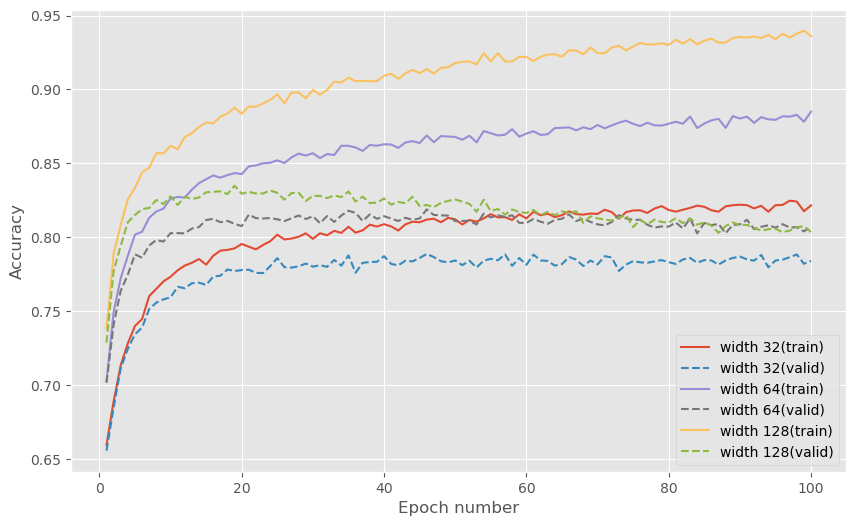
\includegraphics[width=\linewidth]{figures/accuracy.png}
        \caption{accuracy by epoch}
        \label{fig:width_acccurves}
    \end{subfigure} 
    \begin{subfigure}{\linewidth}
        \centering
        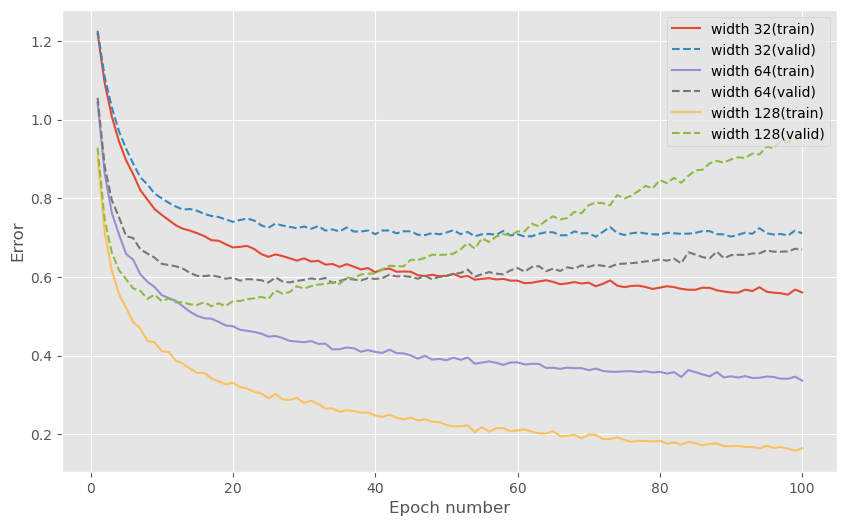
\includegraphics[width=\linewidth]{figures/error.png}
        \caption{error by epoch}
        \label{fig:width_errorcurves}
    \end{subfigure} 
    \caption{Training and validation curves in terms of classification accuracy (a) and cross-entropy error (b) on the EMNIST dataset for different network widths.}
    \label{fig:width}
\end{figure} 
}
}

%% Question Figure 3:
\newcommand{\questionFigureThree} {
\youranswer{Question Figure 3 - Replace these images with figures depicting the accuracy and error, training and validation curves for your experiments varying the number of hidden layers.
%
\begin{figure}[t]
    \centering
    \begin{subfigure}{\linewidth}
        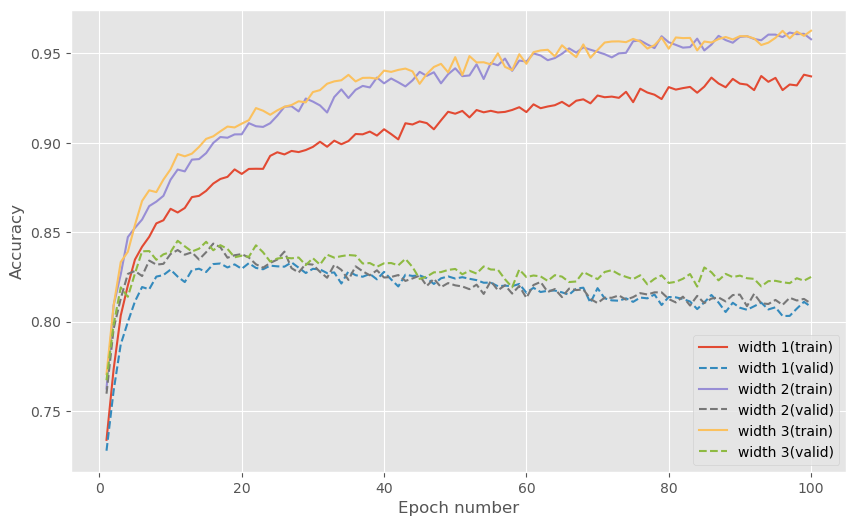
\includegraphics[width=\linewidth]{figures/acc_layers.png}
        \caption{accuracy by epoch}
        \label{fig:depth_acccurves}
    \end{subfigure} 
    \begin{subfigure}{\linewidth}
        \centering
        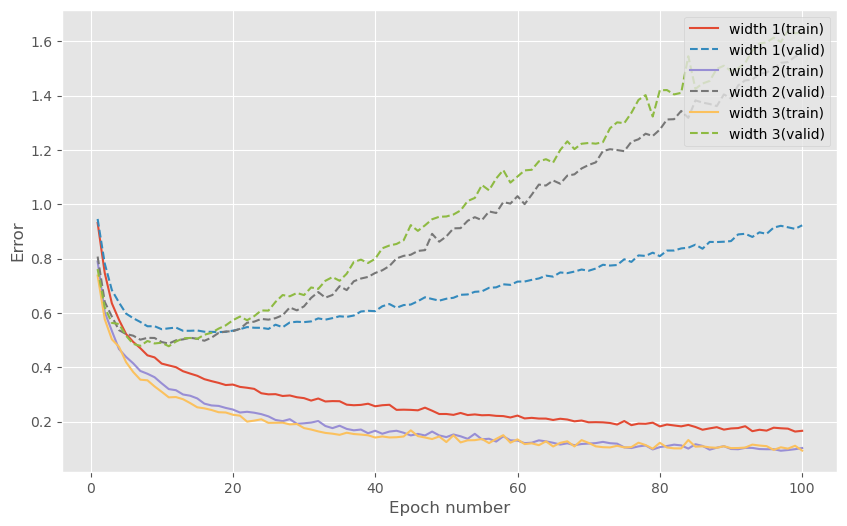
\includegraphics[width=\linewidth]{figures/error_layers.png}
        \caption{error by epoch}
        \label{fig:depth_errorcurves}
    \end{subfigure} 
    \caption{Training and validation curves in terms of classification accuracy (a) and cross-entropy error (b) on the EMNIST dataset for different network depths.}
    \label{fig:depth}
\end{figure} 
}
}

%% Question Figure 4:
\newcommand{\questionFigureFour} {
\youranswer{Question Figure 4 - Replace these images with figures depicting the Validation Accuracy and Generalisation Gap (difference between validation and training error) for each of the experiment results varying the Dropout inclusion rate, and L1/L2 weight penalty depicted in Table 3 (including any results you have filled in).
%
\begin{figure*}[t]
    \centering
    \begin{subfigure}{.475\linewidth}
        \includegraphics[width=\linewidth]{figures/empty_dropout_plot.png}
        \caption{Accuracy and error by inclusion probability.}
        \label{fig:dropoutrates}
    \end{subfigure} 
    \begin{subfigure}{.475\linewidth}
        \centering
        \includegraphics[width=\linewidth]{figures/empty_wd_plot.png}
        \caption{Accuracy and error by weight penalty.}
        \label{fig:weightrates}
    \end{subfigure} 
    \caption{Accuracy and error by regularisation strength of each method (Dropout and L1/L2 Regularisation).}
    \label{fig:hp_search}
\end{figure*}
}
}

%% - - - - - - - - - - - - TABLES - - - - - - - - - - - - 

%% Question Table 1:
\newcommand{\questionTableOne} {
\youranswer{
Question Table 1 - Fill in Table 1 with the results from your experiments varying the number of hidden units.
%
\begin{table}[t]
    \centering
    \begin{tabular}{c|ccc}
    \toprule
        \# Hidden Units & Val. Acc. & Train Error & Val. Error\\
    \midrule
         32            &    78.4\%   &  0.561 &   0.711            \\
         64            &    80.7\%   &  0.336   &   0.670               \\
         128           &    80.4\%   &  0.164  &   0.957           \\ 
    \bottomrule
    \end{tabular}
    \caption{Validation accuracy (\%) and training/validation error (in terms of cross-entropy error) for varying network widths on the EMNIST dataset.}
    \label{tab:width_exp}
\end{table}
}
}

%% Question Table 2:
\newcommand{\questionTableTwo} {
\youranswer{
Question Table 2 - Fill in Table 2 with the results from your experiments varying the number of hidden layers.
%
\begin{table}[t]
    \centering
    \begin{tabular}{c|ccc}
    \toprule
        \# Hidden Layers & Val. Acc. & Train Error & Val. Error \\
    \midrule
         1               &      82.5\%      &   0.444 & 0.551                \\
         2               &      81.0\%      &   0.103 & 1.55                \\
         3               &      82.5\%      &   0.0936 & 1.63                \\ 
    \bottomrule
    \end{tabular}
    \caption{Validation accuracy (\%) and training/validation error (in terms of cross-entropy error) for varying network depths on the EMNIST dataset.}
    \label{tab:depth_exps}
\end{table}
}
}

%% Question Table 3:
\newcommand{\questionTableThree} {
\youranswer{
Question Table 3 - Fill in Table 3 with the results from your experiments for the missing hyperparameter values for each of L1 regularisation, L2 regularisation, Dropout and label smoothing (use the values shown on the table).
%
\begin{table*}[t]
    \centering
    \begin{tabular}{c|c|ccc}
    \toprule
        Model    &  Hyperparameter value(s) & Validation accuracy & Train Error & Validation Error \\
    \midrule
    \midrule
        Baseline &  -                    &               0.837 &       0.241 &  0.533          \\
    \midrule
        \multirow{4}*{Dropout}
                 & 0.6                   &  80.7                &      0.549 & 0.593     \\
                 & 0.7 & --.- & -.--- & -.---  \\
                 & 0.85 & 85.1 &  0.329 &  0.434 \\
                 & 0.97 & 85.4 &  0.244 & 0.457  \\
    \midrule
        \multirow{4}*{L1 penalty}
                 & 5e-4 & 79.5 & 0.642 & 0.658 \\
                 & 1e-3 & --.- & -.--- & -.--- \\
                 & 5e-3 & 2.41 & 3.850 & 3.850 \\
                 & 5e-2 & 2.20 & 3.850 & 3.850 \\
    \midrule
        \multirow{4}*{L2 penalty}  
                 & 5e-4 & 85.1 & 0.306 & 0.460 \\
                 & 1e-3 & --.- & -.--- & -.--- \\
                 & 5e-3 & 81.3 & 0.586 & 0.607 \\
                 & 5e-2 & 39.2 & 2.258 & 2.256  \\
    \midrule
        Label smoothing & 0.1 & --.- & -.--- & -.--- \\
    \bottomrule
    \end{tabular}
    \caption{Results of all hyperparameter search experiments. \emph{italics} indicate the best results per series (Dropout, L1 Regularisation, L2 Regularisation, Label smoothing) and \textbf{bold} indicates the best overall.}
    \label{tab:hp_search}
\end{table*}
}
}

%% END of YOUR ANSWERS